\documentclass[aspectratio=169,10pt]{beamer}
\usepackage[T1]{fontenc}
\usepackage[utf8]{inputenc}
\usepackage[spanish,es-noquoting]{babel}
\usepackage{lmodern,amsmath,amssymb,mathtools,booktabs,graphicx}
\usepackage{xcolor}
\usepackage{listings}
\definecolor{navy}{HTML}{183047}
\definecolor{teal}{HTML}{286A72}
\definecolor{muted}{HTML}{4A5B67}
\definecolor{paperbg}{HTML}{F8FAFB}
\setbeamercolor{normal text}{fg=navy,bg=white}
\setbeamercolor{frametitle}{fg=white,bg=navy}
\setbeamercolor{title}{fg=navy}
\setbeamercolor{structure}{fg=teal}
\setbeamercolor{block title}{fg=white,bg=navy}
\setbeamercolor{block body}{fg=navy,bg=paperbg}
\setbeamertemplate{navigation symbols}{}
\setbeamertemplate{footline}{\leavevmode\hfill\scriptsize AKO (2026) | MIT 05.05.2026 \hspace{1.2em}\insertframenumber\,/\,\inserttotalframenumber\hspace{1.3em}\vspace{0.5em}}
\setbeamertemplate{itemize item}{\color{teal}$\blacktriangleright$}
\setbeamersize{text margin left=0.8cm,text margin right=0.8cm}
\setlength{\parskip}{0.25em}
\newcommand{\X}{X_t}
\newcommand{\aip}{\tau_A}
\newcommand{\slidenote}[1]{\vspace{0.4em}{\footnotesize\color{muted}#1}}
\newcommand{\shortref}[1]{{\footnotesize\color{muted}#1}}
\title[Knowledge Collapse]{AI, Human Cognition and Knowledge Collapse}
\subtitle{Acemoglu, Kong y Ozdaglar (2026)\\Análisis económico, auditoría y formalización Lean}
\author{Alejandro Ventura}
\institute{Artificial Intelligence and Economic Modeling\\Universidad del Pacífico}
\date{Versión del MIT: 5 de mayo de 2026}
\begin{document}

\begin{frame}
  \titlepage
  \vspace{-0.6em}
  \centering\scriptsize\url{https://github.com/alejandroventuraventurameza-tech/ai-04-acemoglu}
\end{frame}

\begin{frame}{Pregunta y resultado: una externalidad de aprendizaje}
\begin{block}{Pregunta}
¿Puede una IA que mejora las decisiones individuales reducir el esfuerzo que sostiene el conocimiento colectivo?
\end{block}
\begin{itemize}
\item El esfuerzo humano produce simultáneamente una señal privada y otra pública.
\item La IA agéntica entrega información \emph{contextual} que sustituye a la señal privada.
\item Nadie internaliza completamente el beneficio social de la señal pública.
\end{itemize}
\[
\text{más precisión de IA}\ \Longrightarrow\
\text{menor esfuerzo privado}\ \Longrightarrow\
\text{menos aprendizaje colectivo}.
\]
\slidenote{La flecha dinámica es condicional: el colapso requiere una elasticidad suficientemente elevada y otras restricciones del modelo.}
\end{frame}

\begin{frame}{Producción: por qué importan ambos tipos de conocimiento}
Sea $a_G,a_I\in\{0,1\}$ el acierto en la predicción general y contextual:
\[
f(a_G,a_I)=f(0,0)+\Delta_G a_G+\Delta_I a_I+\Delta_X a_Ga_I.
\]
\begin{align*}
\Delta_G&=f(1,0)-f(0,0),\\
\Delta_I&=f(0,1)-f(0,0),\\
\Delta_X&=f(1,1)-f(1,0)-f(0,1)+f(0,0).
\end{align*}
\begin{block}{Supuesto 1 del artículo}
$\boxed{\Delta_I=0,\qquad \Delta_X>0.}$
\end{block}
\slidenote{El conocimiento contextual aislado no añade producción. Esta hipótesis es decisiva para que $X=0$ absorba la economía. MIT, p. 9.}
\end{frame}

\begin{frame}{Información: precisiones gaussianas y esfuerzo}
\begin{columns}[T,onlytextwidth]
\column{0.50\textwidth}
\textbf{Señal privada:}
\[
Y_{i,t}=\sigma^{-2}+\lambda_Ie_{i,t}+\aip.
\]
\begin{itemize}
\item $\sigma^{-2}$: precisión a priori.
\item $\lambda_Ie_{i,t}$: aprendizaje humano.
\item $\aip$: recomendación de IA.
\end{itemize}
\column{0.47\textwidth}
\textbf{Señal pública:}
\[
X_{t+1}^{-1}=
(X_t+\lambda_G E_t)^{-1}+\Sigma^2.
\]
\begin{itemize}
\item $E_t=I e_t$ en equilibrio simétrico.
\item $\Sigma^2$: varianza de innovación general.
\item La inversión pública cognitiva es un subproducto del esfuerzo.
\end{itemize}
\end{columns}
\vspace{0.6em}
\[
G(z)=2\Phi(\sqrt z)-1,\quad
g(z)=G'(z)=\frac{\phi(\sqrt z)}{\sqrt z},\qquad z>0.
\]
\end{frame}

\begin{frame}{El problema estático del individuo}
Bajo el Supuesto 1, para $\varepsilon>0$:
\[
\max_{e\ge0}\;
U(e;X,\aip)=
\Delta_G G(X)+\Delta_X G(X)G(Y)
-\frac{\varepsilon}{\varepsilon+1}e^{(\varepsilon+1)/\varepsilon},
\]
\[
Y=\sigma^{-2}+\lambda_Ie+\aip.
\]
En el óptimo interior:
\[
\boxed{\Delta_XG(X)\lambda_Ig(Y)=e^{1/\varepsilon}.}
\]
\begin{itemize}
\item Beneficio marginal: productividad de la precisión contextual.
\item Costo marginal: $e^{1/\varepsilon}$.
\item El individuo toma $X$ como dado: no recibe el beneficio futuro de su contribución pública.
\end{itemize}
\slidenote{La expresión igualada a cero es una FOC, no una función objetivo que deba maximizarse; corrección explícita de una extracción automática anterior.}
\end{frame}

\begin{frame}{Observación 1: dos derivadas cruzadas, dos signos}
Como $g'(z)=-g(z)(1+z)/(2z)<0$ para $z>0$:
\[
\boxed{U_{eX}=\Delta_X\lambda_Ig(X)g(Y)>0}
\]
\[
\boxed{U_{e\tau_A}=\Delta_X\lambda_IG(X)g'(Y)<0.}
\]
\begin{block}{Las condiciones importan}
$X>0$, $\Delta_X>0$, $\lambda_I>0$, $\sigma^{-2}>0$,
$e\ge0$, $\aip\ge0$ y $g(z)>0$ para $z>0$.
\end{block}
Más conocimiento \emph{general} complementa el esfuerzo; más precisión de la IA \emph{contextual} lo sustituye.
\shortref{Fuente: MIT, §3.4, pp. 14--15.}
\end{frame}

\begin{frame}{Observación 2: de la FOC a las decisiones}
Para $e>0$, la curvatura de la utilidad en esfuerzo es:
\[
U_{ee}=\Delta_XG(X)\lambda_I^2g'(Y)
-\frac{1}{\varepsilon}e^{1/\varepsilon-1}<0.
\]
Aplicando el teorema de la función implícita a $U_e=0$:
\[
\frac{\partial e}{\partial X}
=-\frac{U_{eX}}{U_{ee}}>0,
\qquad
\frac{\partial e}{\partial\tau_A}
=-\frac{U_{e\tau_A}}{U_{ee}}<0.
\]
\begin{itemize}
\item Unicidad e interioridad justifican pasar de las diferencias cruzadas a la mejor respuesta.
\item En $X=0$, $e(0,\tau_A)=0$: la monotonía en $\tau_A$ no es estricta allí.
\end{itemize}
\end{frame}

\begin{frame}{Dinámica: cuándo el esfuerzo mantiene el conocimiento}
Con esfuerzo simétrico $e(X,\aip)$:
\[
F(X)=\left[\Sigma^2+
\bigl(X+\lambda_GI\,e(X,\aip)\bigr)^{-1}\right]^{-1}.
\]
Definamos la cantidad de esfuerzo que \emph{mantiene} la precisión:
\[
e_m(X)=\frac{\Sigma^2X^2}{\lambda_GI(1-\Sigma^2 X)},
\quad 0<X<\Sigma^{-2}.
\]
\[
\boxed{F(X)>X\ \Longleftrightarrow\ e(X,\aip)>e_m(X).}
\]
\begin{block}{Interpretación}
El conocimiento colectivo crece únicamente cuando el esfuerzo elegido supera el nivel necesario para compensar la depreciación informacional.
\end{block}
\slidenote{$e_m$ es una herramienta analítica de este repositorio, no una definición original de los autores.}
\end{frame}

\begin{frame}{Por qué el umbral crítico es $\varepsilon=4$}
Cerca de $X=0$, la precisión general tiene un comportamiento de raíz:
\[
G(X)\sim\sqrt{2/\pi}\,X^{1/2}
\quad\Longrightarrow\quad
e(X,\aip)\asymp X^{\varepsilon/2}.
\]
Mientras tanto:
\[
e_m(X)\asymp X^2.
\]
\begin{center}
\begin{tabular}{lll}
\toprule
Régimen & Comparación local & $X=0$\\
\midrule
$0<\varepsilon<4$ & $X^{\varepsilon/2}\gg X^2$ & Inestable\\
$\varepsilon>4$ & $X^{\varepsilon/2}\ll X^2$ & Estable\\
$\varepsilon=4$ & Importan las constantes & Caso límite\\
\bottomrule
\end{tabular}
\end{center}
\slidenote{La teoría dinámica se explica, pero no afirmamos haber formalizado íntegramente el Lema 2 en Lean.}
\end{frame}

\begin{frame}{Ejercicio computacional: mejor respuesta y mantenimiento}
\begin{center}
\IfFileExists{figures/fig2_effort_vs_maintenance.pdf}{
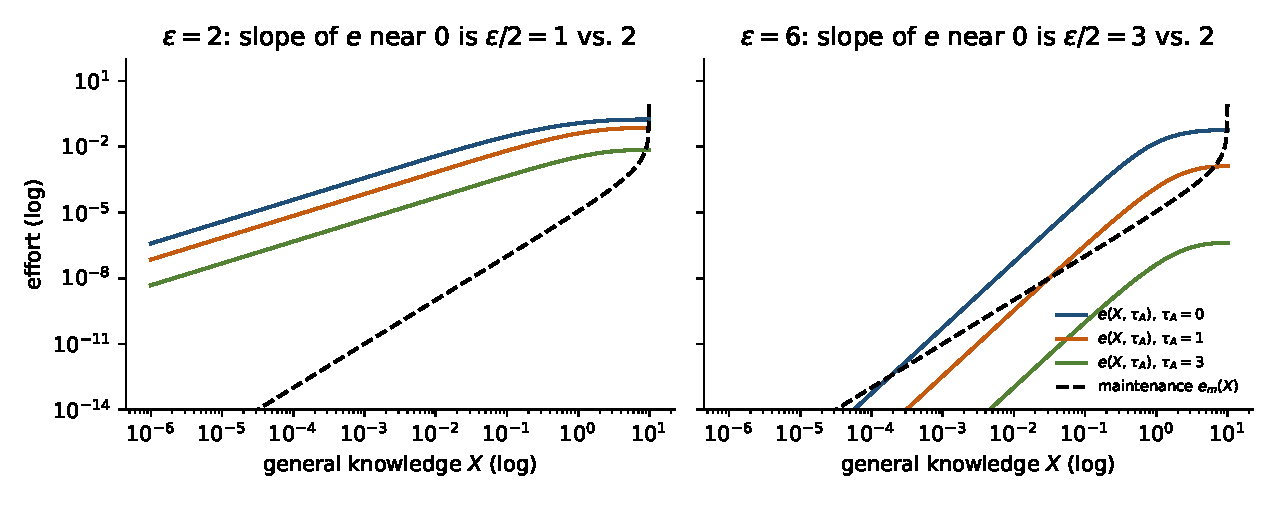
\includegraphics[width=0.84\linewidth,height=0.73\textheight,keepaspectratio]{figures/fig2_effort_vs_maintenance.pdf}
}{
\fbox{\parbox{0.78\linewidth}{Gráfico reproducible: \texttt{python sim/fig\_static.py}}}
}
\end{center}
\slidenote{Figura: cálculos propios con \texttt{sim/model.py}; parámetros ilustrativos, no estimación. Los cruces con $e_m$ corresponden a estados estacionarios positivos.}
\end{frame}

\begin{frame}{La trampa del bienestar: precisión no equivale a mejora social}
\begin{center}
\IfFileExists{figures/fig4_welfare_hump.pdf}{
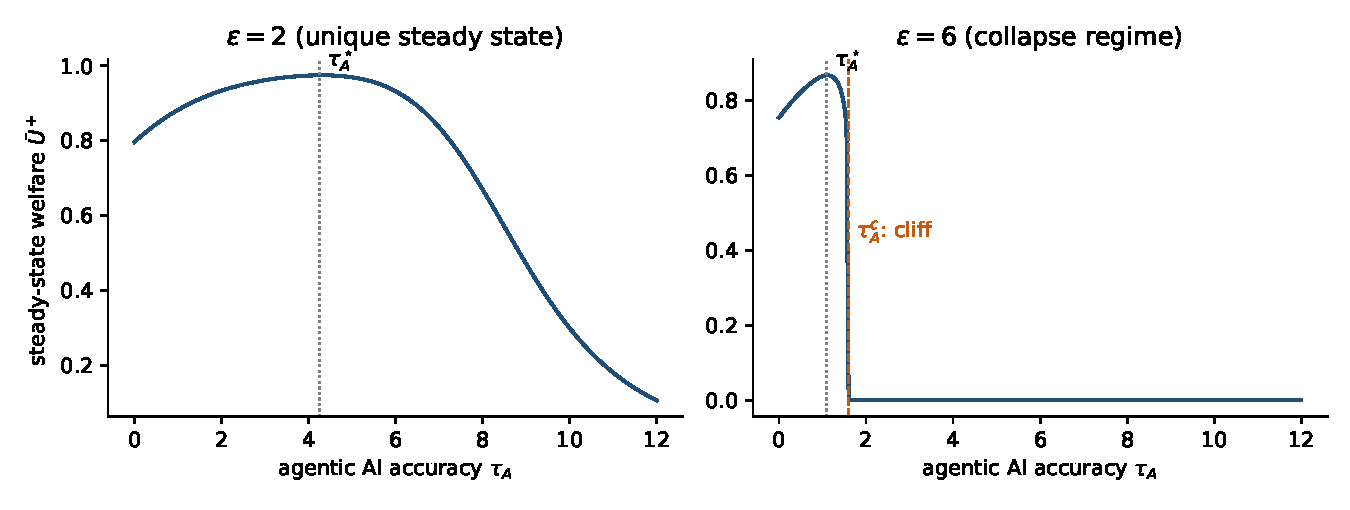
\includegraphics[width=0.85\linewidth,height=0.65\textheight,keepaspectratio]{figures/fig4_welfare_hump.pdf}
}{
\fbox{\parbox{0.78\linewidth}{Gráfico reproducible: \texttt{python sim/welfare.py}}}
}
\end{center}
\[
\underbrace{\frac{d\overline U}{d\tau_A}}_{\text{efecto total}}
=\underbrace{\text{ganancia informacional directa}}_{>0}
+\underbrace{\text{pérdida por menor aprendizaje}}_{<0}.
\]
\slidenote{Proposiciones 10--11: el resultado de un máximo interior exige el Supuesto 2, $\sigma^{-2}\ge\sqrt2-1$, además de las condiciones del régimen dinámico.}
\end{frame}

\begin{frame}{El experimento de falsación: ¿el planificador también pierde?}
\begin{columns}[T,onlytextwidth]
\column{0.49\textwidth}
\textbf{Equilibrio descentralizado}\\[0.5em]
\begin{itemize}
\item Cada cohorte ignora el valor futuro de su señal pública.
\item Aumentar $\tau_A$ reduce el esfuerzo.
\item El bienestar estacionario puede ser no monótono.
\end{itemize}
\column{0.49\textwidth}
\textbf{Planificador social}\\[0.5em]
\begin{itemize}
\item Puede mantener la misma trayectoria de esfuerzo.
\item Una señal más precisa no empeora decisiones óptimas.
\item Su valor es no decreciente en $\tau_A$.
\end{itemize}
\end{columns}
\begin{block}{Alcance del argumento}
Comparación de valores óptimos con información Blackwell-superior y trayectorias factibles anidadas; no es una demostración del equilibrio descentralizado.
\end{block}
\end{frame}

\begin{frame}{Extensión propia: $\Delta_I>0$ elimina el colapso completo}
Relajamos una hipótesis de producción del artículo, manteniendo las mismas señales:
\[
\underbrace{(\Delta_I+\Delta_X G(X))\lambda_Ig(Y)}_{\text{beneficio marginal}}
=e^{1/\varepsilon},\qquad \Delta_I>0.
\]
Entonces, aun si $X=0$, hay incentivo privado a aprender:
\[
e(0,\tau_A)>0\quad\Longrightarrow\quad F(0)>0.
\]
\begin{itemize}
\item No hay punto fijo de colapso total en cero para precisión de IA finita.
\item Puede persistir un equilibrio con poco conocimiento y una curva de bienestar interior.
\item El cálculo es una extensión analítica y numérica, \emph{no} un resultado demostrado por el artículo.
\end{itemize}
\end{frame}

\begin{frame}[fragile]{Lean: de una afirmación económica a una prueba verificable}
\textbf{Enunciado matemático del motor de sustitución:}
\[
g(\tau)=\frac{e^{-\tau/2}}{\sqrt{2\pi\tau}},\quad
\tau>0;\qquad
g(\tau)>0,\quad \tau_1<\tau_2\Rightarrow g(\tau_2)<g(\tau_1).
\]
\textbf{Traducción en el repositorio:}
\begin{lstlisting}[basicstyle=\ttfamily\scriptsize,breaklines=true]
def t1SubstitutionEngineSpec : Prop := ...
theorem t1SubstitutionEngine_holds :
    t1SubstitutionEngineSpec := by
  constructor
  ...
  exact Real.rpow_lt_rpow_of_neg ha hab (by norm_num)
\end{lstlisting}
\begin{block}{Qué se comprueba}
La potencia de exponente negativo es decreciente; la prueba combina este hecho con la positividad y monotonía de $\exp(-\tau/2)$. T1 compiló y pasó la auditoría de axiomas.
\end{block}
\slidenote{Fuente: \texttt{ProofInterface.lean} (extracto).}
\end{frame}

\begin{frame}{El límite de la formalización: especificación versus artículo}
\begin{tabular}{p{0.26\linewidth}p{0.62\linewidth}}
\toprule
Objeto & Qué dice realmente Lean\\
\midrule
T1 & Positividad y antitonicidad de la función gaussiana concreta $g_{\rm AKO}$.\\[0.5em]
T2 & Signos y diferencias de la Observación 1 \emph{condicionados} a \texttt{AccuracyAssumptions} de $G,g,g'$.\\[0.5em]
T3, T4, T6, T7 & Se añadieron pruebas de raíces de la FOC, mantenimiento, frontera en cero y valor del planificador; ver el informe de validación.\\
\bottomrule
\end{tabular}
\vspace{0.7em}
\begin{block}{Cuidado semántico}
T2 no demuestra por sí solo que la función concreta de precisión gaussiana satisface todas las hipótesis, ni prueba el umbral dinámico $\varepsilon=4$. Eso exige obligaciones adicionales.
\end{block}
\end{frame}

\begin{frame}{Auditoría manuscrita: no confiar ciegamente en la IA}
\IfFileExists{hand/ai-04.pdf}{
  \begin{center}
  \includegraphics[page=3,width=0.96\linewidth,height=0.69\textheight,keepaspectratio]{hand/ai-04.pdf}
  \end{center}
  \slidenote{Derivación original, p.~3. Veredicto (p.~6): la extracción confundió la FOC con la función objetivo; los signos de la Observación 1 son correctos.}
}{
  \begin{block}{Evidencia revisada, PDF pendiente de incorporación a GitHub}
  La derivación corregida de seis páginas contiene ambos signos y la extensión de desplazamiento parcial. Se verificó el denominador $U_{ee}$ en p.~4.
  \end{block}
  \[
  g'(\tau)=-\frac{1+\tau}{2\tau}g(\tau),\qquad
  U_{eX}>0,\quad U_{e\tau_A}<0.
  \]
  \slidenote{La extracción previa confundió la FOC con el objetivo; no es un error del artículo. El PDF corregido debe incorporarse en \texttt{hand/ai-04.pdf}.}
}
\end{frame}

\begin{frame}{Reproducibilidad y estado de auditoría}
\textbf{Comandos de comprobación:}
\begin{itemize}
\item \texttt{python sim/verify\_static.py}: identidades simbólicas de la estática.
\item \texttt{python sim/fig\_static.py}: figuras 1--3.
\item \texttt{python sim/welfare.py}: figuras 4--8.
\item \texttt{cd extra/standalone-lean \&\& lake build}: prueba kernel del proyecto Lean autónomo.
\end{itemize}
\begin{block}{Resultado de verificación y alcance}
Flujo oficial: \texttt{check --fast}, compilación del módulo y siete comprobaciones de axiomas aprobadas (run 45554882759). Carpeta generada en \texttt{lean/}. El alcance es parcial; no se certifica el artículo completo. La evidencia manuscrita debe figurar en el repositorio.
\end{block}
\end{frame}

\begin{frame}{Conclusión}
\begin{enumerate}
\item La IA puede elevar el acierto privado y reducir la inversión en conocimiento público: hay una \textbf{externalidad intertemporal}.
\item La distinción formal es $U_{eX}>0$ frente a $U_{e\tau_A}<0$, bajo hipótesis explícitas.
\item El umbral $\varepsilon=4$ es una comparación de tasas de desaparición del esfuerzo y de su nivel de mantenimiento.
\item La hipótesis $\Delta_I=0$ es decisiva; la relajación $\Delta_I>0$ permite evaluar la fragilidad del colapso.
\item La formalización verifica \textbf{enunciados concretos}, no automáticamente toda la interpretación económica.
\end{enumerate}
\vspace{0.4em}
\shortref{Fuente primaria: Acemoglu, Kong y Ozdaglar (2026), versión MIT 05.05.2026. Código y figuras: repositorio del estudiante.}
\end{frame}
\end{document}
